\documentclass[a4paper,twoside]{article}

\usepackage{epsfig}
\usepackage{tabularx}
\newcolumntype{Y}{>{\raggedright\arraybackslash}X}
\usepackage{subcaption}
\usepackage{calc}
\usepackage{amssymb}
\usepackage{amstext}
\usepackage{amsmath}
\usepackage{amsthm}
\usepackage{multicol}
\usepackage{pslatex}
\usepackage[utf8]{inputenc}
\usepackage{apalike}
\usepackage{algorithm2e}
\usepackage[bottom]{footmisc}
\usepackage{placeins}
\usepackage{SCITEPRESS}     % Please add other packages that you may need BEFORE the SCITEPRESS.sty package.

\begin{document}

\title{A Multimodal Sensor--HAR--Language Architecture for Goal-Aware User Interaction in Edge--Fog Smart Environments}

\author{\authorname{First Author Name\sup{1}, Second Author Name\sup{1} and Third Author Name\sup{2}}
\affiliation{\sup{1}Institute of Problem Solving, XYZ University, My Street, MyTown, MyCountry}
\affiliation{\sup{2}Department of Computing, Main University, MySecondTown, MyCountry}
\email{\{first\_author, second\_author\}@ips.xyz.edu, third\_author@dc.mu.edu}
}

\keywords{Smart environments, Face recognition, Social robots, Human activity recognition, Edge--fog computing, Large language models, Context-aware interaction.}

\abstract{In a shared home, a conversational assistant must relate a resident's request to the right person, time period and source of evidence. We propose a four-layer reference architecture that connects multimodal sensing and human activity recognition (HAR) to goal-aware dialogue. The layers exchange evidence with explicit provenance and temporal scope, distinguishing sensor observations, activity estimates and user statements. A household prototype uses Reachy Mini for camera-based session selection and draws on ultra-wideband localisation, wearable measurements and ambient sensors for activity context. A locally hosted language model serves three roles in sequence, selecting metric queries, assembling context and generating replies. In a four-person household, the face recognition trial yielded 48 correct outcomes in 50 attempts (96\%). We examined 50 scripted user turns against 72 hours of household sensor data and used a separate paired test to examine retrieval of details carried by contextual events. The case study illustrates how an assistant can use recent and historical evidence in the same exchange, and where it needs to verify the source or time period before answering.}

\onecolumn \maketitle \normalsize \setcounter{footnote}{0} \vfill

\section{\uppercase{Introduction}}
\label{sec:introduction}

A resident may ask a home assistant about exercise earlier that morning, correct its interpretation of a recent activity or request a suggestion that fits a stated preference. Each request depends on evidence that the home may only partially observe. Ambient devices and wearables offer complementary views of daily life~\cite{cook2007smart}, and Hong, Nugent and colleagues showed how to combine observations of uncertain reliability when inferring activities~\cite{hong2009evidential}. Edge--fog computing enables devices and nearby servers to share the work of collecting and interpreting these observations~\cite{shi2016edge}. A social robot provides an embodied interface through which residents can use the resulting services~\cite{broadbent2009acceptance}.

Human activity recognition (HAR) relates patterns in sensor data to descriptions of behaviour~\cite{bulling2014tutorial}. Data-driven methods learn these patterns from examples~\cite{ordonez2016deep}, while knowledge-driven methods encode relationships among observations, context and activities~\cite{polo2025health}. In a shared home, activity recognition and attribution pose separate questions. A contact sensor may indicate that a cupboard opened, while localisation and proximity can provide evidence about which occupant was involved~\cite{poloMultiOccupancy,polo2024social}. The assistant must preserve this distinction when it describes the event.

Large language models (LLMs) can interpret conversational references and formulate responses using environmental context. Recent systems use sensory evidence to decide whether assistance is warranted, select tools or adapt how a suggestion is presented~\cite{yin2025harmony,yang2025contextagent,yang2026proagent,lee2025sensible}. In a household dialogue, the model may need to bring together evidence from different periods and resolve a reference to a particular resident, activity or device. A correction also changes what the assistant should say, even when the underlying sensor record stays the same. We use \emph{goal-aware dialogue} to mean that a goal stated by the user, such as becoming more active, can guide a relevant and optional suggestion.

Our contribution is a four-layer reference architecture that links sensing and HAR to dialogue through interfaces for identity, time-scoped queries and contextual events. A local prototype uses face recognition to select a session and assigns metric resolution, context selection and reply generation to separate roles. The case study examines target-user recognition, evidence use in scripted dialogue and the contribution of structured events to detail retrieval.

Section~\ref{sec:related} reviews prior work. Section~\ref{sec:methodology} describes the architecture and deployment, and Section~\ref{sec:case-study} presents the household case study. Section~\ref{sec:evaluation} reports the evaluation, followed by discussion and conclusions in Section~\ref{sec:discussion}.

\section{\uppercase{Related Work}}
\label{sec:related}

Three lines of work inform the proposed architecture. Smart-home middleware provides access to heterogeneous devices, sensing and robotics connect those devices to activities and people, and LLM agents use the resulting context to decide what assistance to offer.

\subsection{Smart-Home Middleware, Sensing and Robotics}

The Context Toolkit separated the acquisition and representation of context from its use by applications~\cite{dey2001toolkit}. The Gator Tech Smart House and HomeOS applied this principle to residential settings through abstractions for devices and services~\cite{helal2005gator,dixon2012homeos}. Work on universAAL added explicit semantics for assistive services~\cite{zmuda2016universaal}. These systems established mechanisms for sharing context across applications.

CASAS used timestamped residential events to study activities over time~\cite{cook2013casas}, while SPHERE brought environmental, wearable and video measurements into a common sensing infrastructure~\cite{elsts2018sphere}. Social robots provide a way to act on this context in direct exchanges with occupants. Robot-Era evaluated the acceptance of assistive robot services~\cite{cavallo2018robotera}, and CloudIA examined engagement with personalised robot-mediated activities~\cite{sorrentino2023cloudia}. Reachy Mini provides a camera and audio interface within a single platform~\cite{danieau2026reachymedia}. For visual identification, work on video face recognition shows how a system can aggregate evidence across frames while assigning greater weight to informative views~\cite{yang2017nan}.

\subsection{LLM Agent Architectures for Smart Environments}
\label{subsec:related-llm}

Language models can contribute to activity recognition or use the results of an independent recogniser. SensorLLM aligns motion signals with language for activity recognition~\cite{li2025sensorllm}. Polo-Rodr\'iguez et al.~\cite{polo2025chatbots} use indoor localisation, ambient sensing and HAR to supply activity and location context to a chatbot. The latter approach lets dialogue use information produced by services with their own observation windows and methods.

Harmony is a close architectural precedent. It separates event interpretation, decision-making and appliance control around a local model, with evaluation in a virtual environment and an exploratory user study~\cite{yin2025harmony}. ContextAgent draws on egocentric sensing and user information to decide when assistance is warranted and which tools to invoke. Its benchmark includes a subset of cases with raw sensory inputs~\cite{yang2025contextagent}. ProAgent addresses the overhead of continuous egocentric sensing by using inexpensive cues to trigger richer perception. Its evaluation uses everyday recordings and participant feedback on the resulting assistance~\cite{yang2026proagent}. Sensible Agent adapts the content and modality of augmented-reality suggestions and lets users confirm or modify them. Its controlled laboratory study used experimenter-triggered assistance to examine how the interaction was received~\cite{lee2025sensible}.

Goals and tool use add another dimension to this comparison. Sasha translates high-level goals into actions on home devices~\cite{king2024sasha}, while SayCan and ReAct illustrate how language-based decisions can incorporate available capabilities or observed tool outputs~\cite{ahn2022saycan,yao2023react}. In assistive dialogue, a resident's stated goal can also guide the content of a suggestion. Its relevance in a given turn and its effects on behaviour over time are distinct outcomes. Longitudinal studies of coaching and adaptive interventions provide methods for investigating the latter~\cite{bickmore2013interventions,nahumshani2018jitai}.

Egocentric systems follow the wearer across settings, while home infrastructure can retain a history of shared spaces and devices. Our architecture draws primarily on that household history and combines it with wearable measurements, visual session selection and information supplied by the resident. This design foregrounds the provenance of evidence that may refer to different people or periods. The studies above provide evidence at different levels, including benchmark decisions, responses to real-world recordings and controlled interaction. Sustained field studies can reveal how these capabilities work together in daily routines~\cite{brown2011wild}. Our case study addresses separate components of that broader evaluation.

\section{\uppercase{Methodology and Materials}}
\label{sec:methodology}

We first specify the responsibilities of the layers and the interfaces through which they exchange evidence and requests. We then describe the devices and computing infrastructure used to instantiate the architecture in a home.

\subsection{Reference Architecture}
\label{subsec:general-architecture}

The four layers are \emph{Sensing and Actuation}, \emph{Edge--Fog Infrastructure}, \emph{Pattern and Action Services}, and \emph{Intelligent Care}. Observations flow upwards to services that interpret them. Queries and proposed actions travel downwards to the appropriate service or device (Figure~\ref{fig:reference}).

\begin{figure}[t]
\centering
\small
\setlength{\fboxsep}{4pt}
\begin{tabular}{@{}c@{}}
\textbf{User} \\
{\footnotesize User input \(\downarrow\quad\uparrow\) Replies and suggestions} \\
\fbox{\parbox{0.89\columnwidth}{\textbf{Intelligent Care}\\Context selection, validation and dialogue}} \\
{\footnotesize Evidence \(\uparrow\quad\downarrow\) Queries and requests} \\
\fbox{\parbox{0.89\columnwidth}{\textbf{Pattern and Action Services}\\Metrics, identity, localisation and activity}} \\
{\footnotesize Observations \(\uparrow\quad\downarrow\) Service requests} \\
\fbox{\parbox{0.89\columnwidth}{\textbf{Edge--Fog Infrastructure}\\Messaging, history and distributed processing}} \\
{\footnotesize Device data \(\uparrow\quad\downarrow\) Device commands} \\
\fbox{\parbox{0.89\columnwidth}{\textbf{Sensing and Actuation}\\Ambient and wearable sensors, camera and robot}} \\
\end{tabular}
\caption{Reference architecture and exchanges between layers. Device types illustrate one possible deployment.}
\label{fig:reference}
\end{figure}

\paragraph{Sensing and Actuation.}
This layer acquires observations from the physical environment and delivers outputs to it. Contact sensors can report discrete events, while wearable, ambient and audiovisual devices can supply streams at different rates. Each observation carries a source and timestamp, together with a subject or location when available. Actuators can report the outcome of a command, allowing subsequent observations to inform the next decision.

\paragraph{Edge--Fog Infrastructure.}
This layer distributes observations, provides access to historical records and allocates processing across devices and nearby servers. Publish--subscribe middleware decouples producers from consumers, as illustrated by MQTT-based fog systems and event distribution in ZeroC Ice deployments~\cite{oasis2019mqtt,zerocIcestorm}. Latency-sensitive filtering can run near acquisition, while aggregation or more demanding inference can run on shared infrastructure. Services use the same observation and query interfaces across these placements.

\paragraph{Pattern and Action Services.}
Pattern services derive quantities and estimates for specific tasks, including identity, localisation and activity recognition. Learned models can capture complex multimodal patterns, although supervised approaches depend on representative labelled data~\cite{ordonez2016deep}. Knowledge-driven rules can incorporate expert judgement and expose the basis of an estimate, but require adaptation to the setting. Fuzzy rules can represent graded support, as in the association of ambient events with nearby occupants~\cite{poloMultiOccupancy}. These approaches share an interface for reporting an estimate, its scope and its supporting evidence. Metric computation is exposed separately so that language generation can use an inspectable result. Action services check feasibility and permissions before execution.

\paragraph{Intelligent Care.}
This layer determines which evidence is relevant to a request, how it relates to the recent dialogue and whether a stated goal should inform the response. A resident can correct an estimate or express a preference about how assistance is offered. Where appropriate, a caregiver or domain expert can help specify meaningful patterns and conditions that warrant human judgement. Recent observations support immediate exchanges, while longer records can inform follow-up questions about recurring activities or longer-term goals.

\subsubsection{Evidence and Temporal Scope}
\label{subsec:evidence-method}

Each evidence item carries a type, a source, a time point or interval and, where available, a subject or region. An \emph{observation} reports a measured value or recorded state. An \emph{inference} interprets one or more observations and can carry its supporting evidence. A \emph{user declaration} records what the person said and when, with a separate time reference when the statement concerns another period. A session identity associates the current exchange with a profile. Assigning a historical observation from a shared device to that profile requires separate evidence.

A historical query specifies a target, an operation and an interval anchored to the time of the current turn. The dialogue history helps resolve expressions such as \emph{then} or \emph{that morning}. The metric service returns the interval actually used, the result and any limits on coverage. A reply can therefore distinguish a sparse record from a well-observed interval and can report uncertainty if the subject or time period remains unresolved.

\subsection{Deployment in a Multimodal Smart Home}

The household prototype combines room estimates and timestamped sensor readings to identify candidate activities. A camera-equipped robot provides the interaction interface and can select the session associated with a recognised resident. Figure~\ref{fig:architecture} shows how the visual and activity paths converge at the dialogue coordinator.

\subsubsection{Sensors and Interaction Devices}
\label{subsec:setup}

Figure~\ref{fig:devices} is reserved for a photograph of the devices used in the deployment.

\begin{itemize}
\item \textbf{Reachy Mini robot.} Its camera supplies face images for session selection, and its microphone and speaker provide the interface for spoken interaction.
\item \textbf{Google Pixel Watch.} A background service on the watch records step counts, heart rate and the system's bedtime-mode flag as updates become available. The watch also provides UWB ranging with FiRa-compatible anchors for room-level localisation~\cite{anguita2025uwb}.
\item \textbf{Indoor localisation.} Qorvo ultra-wideband (UWB) boards provide measurements used to estimate the resident's room.
\item \textbf{Ambient devices.} Aqara Zigbee sensors and other Home Assistant channels record events involving kitchen objects and measurements such as bathroom humidity and television power.
\end{itemize}

\begin{figure}[t]
\centering
\IfFileExists{deployment-devices.pdf}{%
    \includegraphics[width=\columnwidth]{deployment-devices.pdf}%
}{%
    \fbox{\rule{0pt}{20mm}\rule{0.88\columnwidth}{0pt}}%
}
\caption{Sensing and interaction devices used in the household deployment.}
\label{fig:devices}
\end{figure}

\subsubsection{Edge Nodes, Fog Server and Middleware}

Raspberry Pi edge nodes connect to the UWB boards and publish localisation data over MQTT. Home Assistant integrates the ambient channels, and a local broker distributes events to the services that consume them. This arrangement follows the division of sensing and local processing used in MQTT-based fog deployments~\cite{oasis2019mqtt}. A central computer serves as the fog node and runs the Qwen model.

\subsubsection{Context Exchange and Validation}
\label{subsec:agent-methods}

The dialogue coordinator assigns three roles. Metric resolution selects a supported operation and obtains a result for the requested period. Context selection identifies relevant activity estimates, environmental events and user statements. Reply generation combines those inputs with the latest turn and any applicable preference. When a resident corrects an estimate, the declaration can guide subsequent replies while the original observation remains available for inspection.

The reference architecture treats reflexive validation as a design requirement. Before a proposed interpretation guides a reply or action, the system needs a way to check its evidential basis and temporal scope. It can then revise the interpretation, ask for clarification or report insufficient evidence. For device actions, Harmony illustrates how feasibility can be checked before execution~\cite{yin2025harmony}. In our prototype, validation checks the structured operation and evidence selections. The dialogue evaluation examines the text produced from those inputs.

\begin{figure*}[t]
    \centering
    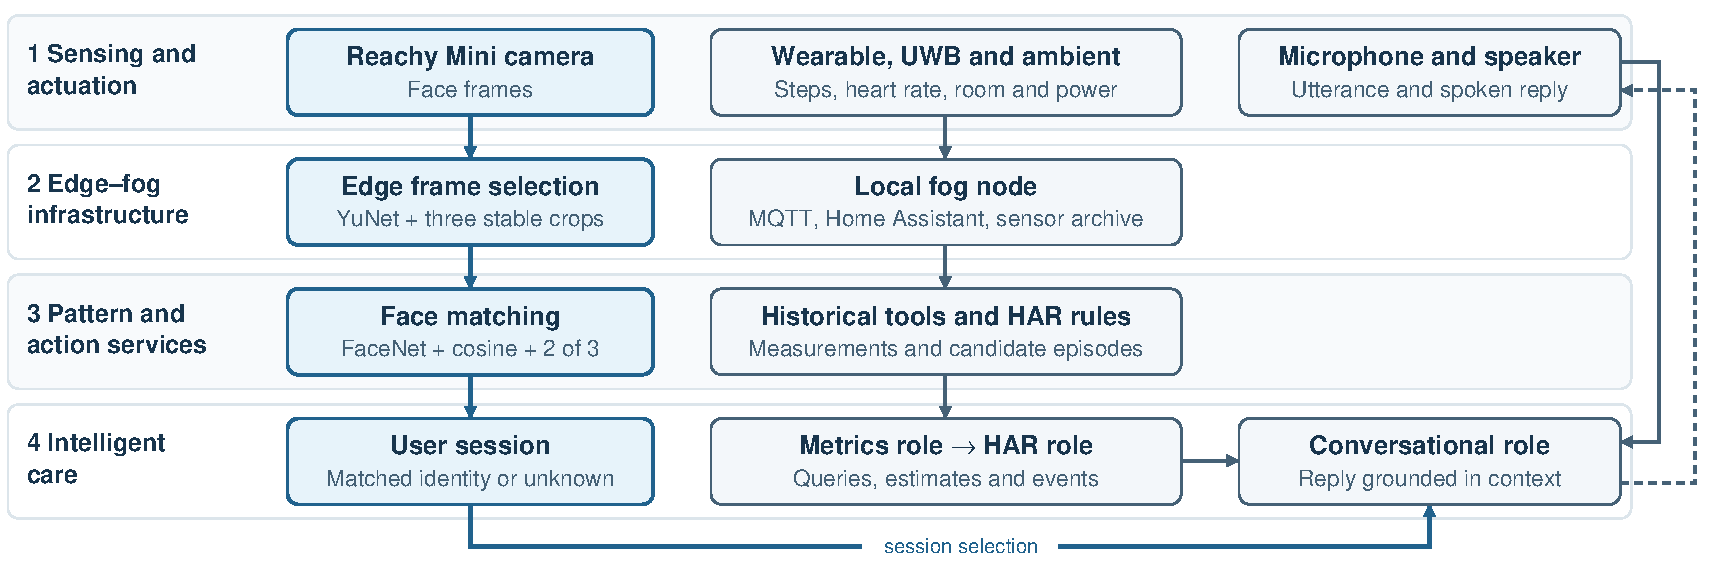
\includegraphics[width=\textwidth]{architecture.pdf}
    \caption{Household implementation of the reference architecture. The blue path connects face frames to session selection. The central path carries measurements and episode candidates. The dashed arrow returns the reply to the robot.}
    \label{fig:architecture}
\end{figure*}


\section{\uppercase{Case Study}}
\label{sec:case-study}

The deployment took place in a four-person household. The target resident was a 43-year-old woman who lived with her spouse and two children. She was the subject of the face recognition trial and the source of the wearable measurements. Figure~\ref{fig:floor-plan} is reserved for the layout of the monitored home.

The sensor archive spans 72 hours, from 31 October 2026 at 12:06 to 3 November 2026 at 12:06 in the Europe/Madrid time zone. The final timestamp is excluded, yielding 4,320 one-minute bins. Table~\ref{tab:coverage} reports the number of bins with a recorded value for each channel. Coverage describes the availability of measurements, which varies with the reporting behaviour of each device.

\begin{figure}[t]
\centering
\IfFileExists{household-floor-plan.pdf}{%
    \includegraphics[width=\columnwidth]{household-floor-plan.pdf}%
}{%
    \fbox{\rule{0pt}{20mm}\rule{0.88\columnwidth}{0pt}}%
}
\caption{Layout of the monitored home.}
\label{fig:floor-plan}
\end{figure}

\begin{table}[t]
\centering
\caption{Recorded values per channel over the three-day household observation period.}
\label{tab:coverage}
\small
\begin{tabular}{@{}lrr@{}}
\hline
Channel & Observed bins & Coverage \\
\hline
Steps & 4,320 & 100.0\% \\
Heart rate & 3,768 & 87.2\% \\
Watch bedtime mode & 4,320 & 100.0\% \\
Room estimate & 2,529 & 58.5\% \\
Television power & 3,384 & 78.3\% \\
Bathroom humidity & 183 & 4.2\% \\
Entrance sensor & 81 & 1.9\% \\
\hline
\end{tabular}
\end{table}

For bathroom humidity and television power, preprocessing stores the trailing median minus the current reading. The windows are two and 24 hours, respectively, and use the available observations, including the current reading. A television power event requires two readings at most five minutes apart, a rise of at least 20~W and a crossing from below to at least 20~W above the rolling median. The shower rule uses a separate comparison with the most recent humidity reading in the hour preceding the observed bathroom episode. It can use a humidity reading recorded up to ten minutes after the last bathroom observation.

\subsection{Reachy Mini Camera and Face Recognition}
\label{subsec:face}

The Reachy Mini client uses OpenCV and YuNet~\cite{wu2023yunet} to detect a single complete face. The default acquisition procedure requires a bounding box of at least 120 pixels per side and an intersection over union of at least 0.65 with the first box. The client collects five distinct frames during a stable acquisition lasting at least one second. It ranks the face crops by a score combining sharpness, exposure and the fraction of clipped pixels, then sends the three highest-ranked crops to a local vision service.

The service aligns each face and obtains a 512-dimensional FaceNet embedding through DeepFace~\cite{schroff2015facenet,serengil2020lightface}. For each frame and enrolled profile, it takes the smallest cosine distance between the crop embedding and the profile's reference embeddings. It ranks profiles by their median distance across at least two valid frames. Acceptance requires a median distance of at most 0.50, a margin of at least 0.05 to the next candidate when one exists, and agreement from at least two individual frame decisions. The service returns an unknown identity when these conditions are unmet.

Acquisition stability limits variation between frames. The distance threshold and margin address weak or ambiguous matches, and the frame agreement requirement reduces the influence of a single crop. When multiple faces are visible, the single-face requirement can delay a decision. The household trial reports aggregate outcomes using these configuration defaults.

\subsection{Local Agent Integration}
\label{subsec:case-agents}

The prototype runs Qwen3-4B-Instruct-2507 in Q4\_K\_M quantisation through Ollama~\cite{qwen2025instruct}. The text evaluation fixes the resident profile and supplies an explicit reference time with each Spanish user turn. The coordinator makes three sequential model calls. The first selects a supported operation from the current turn and recent dialogue, and the metric engine computes the result. The second selects a candidate activity episode or abstains. It can also extract a statement directly from the user turn. The third generates a reply from selected evidence and recent dialogue.

The coordinator checks the structured outputs of the first two roles. The reply instructions require the model to preserve the distinction among measurements, estimates and user statements, and to use the time interval returned by the metric service. The prototype retains the two preceding exchanges and the latest event per source. It marks television power events as recent for ten minutes and user statements for fifteen minutes.

In one scripted exchange, the user says they are reading a novel in another room. At 12:41, the television power rises from 1.0 to 70.6~W. The assistant can refer to both items on later turns. The statement describes what the user reported doing, while the power change describes the appliance. Keeping the sources distinct allows a reply about the television to use the measured change without assigning the user to the room or attributing viewing behaviour to them.

\subsubsection{Historical Queries and Activity Rules}
\label{subsec:case-rules}

The prototype separates the resolution of metric queries from the selection of activity context.

\begin{itemize}
\item \textbf{Metrics agent.} The agent selects a supported query from the user turn and recent dialogue. The metric service resolves relative time expressions against the local calendar and uses observations before the turn's reference time \(t_0\). It computes the step total and mean heart rate from the recorded values in the requested interval. Heart-rate coverage is the fraction of minutes with a reading. Recorded zeros count as observations, while missing values are excluded.

\item \textbf{HAR context agent.} The rule engine generates candidate activity intervals from the sensor record (Table~\ref{tab:rules}). The agent selects the candidate relevant to the turn or leaves the activity unspecified. For most rules, the engine can group matching minutes separated by gaps of up to five minutes. It retains those gaps in the interval and classifies the episode as supported when at least 80\% of its minutes meet the rule. An episode that reaches the query boundary may represent only part of the activity.
\end{itemize}

\begin{table*}[t]
\centering
\caption{Operational rules and interpretation of evidence in the household prototype.}
\label{tab:rules}
\small
\begin{tabularx}{\textwidth}{@{}p{0.17\textwidth}YY@{}}
\hline
\textbf{Rule} & \textbf{Evidence} & \textbf{Interpretation} \\
\hline
Exercise & At least 60 steps/min and at least 100 beats/min in matching minutes, with a minimum candidate window of five minutes & Candidate interval compatible with ambulatory exercise. \\
Rest & Zero recorded steps and at most 65 beats/min in matching minutes, with a minimum candidate window of ten minutes & Rest estimate with reported temporal support. \\
Bathroom or shower & Bathroom room estimate. A shower candidate also requires a humidity rise of at least eight percentage points above the pre-episode reference. & Approximate shower timing based on the bathroom and humidity observations. \\
Kitchen use & Kitchen room estimate and a fridge light reading of at least 10 lux or a glass or plate sensor event in the same minute & Evidence of kitchen use. A user statement can clarify the activity. \\
Watch bedtime & Operating-system mode flag & Recorded start, end or duration of the mode. \\
Entrance & Entrance-area sensor event & Evidence of activity at the entrance, with direction and time away unresolved. \\
\hline
\end{tabularx}
\end{table*}

\subsection{\uppercase{Evaluation}}
\label{sec:evaluation}

The evaluation addresses three questions at different levels. The recognition trial examines whether the camera can identify the target resident (RQ1). The dialogue review examines how replies use evidence across turns (RQ2). The paired event test isolates the effect of supplying a detail in a structured event (RQ3).

\paragraph{Household Recognition}

The target-user trial comprised 50 recognition attempts in a household that included the resident's spouse and two children aged 11 and 14. It yielded 48 correct outcomes (96\%). The available aggregate gives the overall result for this household. It leaves probe composition, acquisition conditions and the distribution of errors unresolved.

\paragraph{Dialogue Evaluation}


The dialogue evaluation comprised 50 scripted user turns grouped into 15 exchanges. Each turn was assigned a reference time within the 72-hour observation period or at its endpoint. The Spanish prompts represent routine situations, including greetings, questions about recent activity, follow-ups about measurements and corrections of activity estimates. Two exchanges introduced goals concerning daily movement and vegetable intake, allowing the model to formulate suggestions in the context of the conversation.

An LLM-assisted rubric review examined the visible replies against the sensor evidence and the preceding dialogue. It checked the use of the requested period and source, the distinction between observations and estimates, and the handling of missing evidence. For quantitative questions, it also checked the reported value against the metric service output. The trace links each reply to the user turn, reference time, selected operation and contextual evidence.

\paragraph{Paired Event-Payload Probe}

The event probe invokes the conversational role twice for each of 12 questions. For each pair, it holds the reference time, model, question, preceding dialogue, metrics and activity context fixed. The conditions differ in whether the event list contains the target event, and their order alternates across pairs. Eight questions ask for a detail from a scripted user statement after two unrelated exchanges. Four ask for the values immediately before and after a recorded change in television power. For the power cases, the fixed metric context includes the current reading and its difference from the rolling median.

The recovery check matches the requested detail in the reply or, for power questions, both values in the requested order. A separate reading of the replies assesses whether the model correctly attributes recovered details and how it responds when the event is withheld.

\begin{table}[t]
\centering
\caption{Paired event-payload probe.}
\label{tab:probe}
\small
\begin{tabularx}{\columnwidth}{@{}Yrr@{}}
\hline
Requested detail & Event kept & Event removed \\
\hline
Prior self-report & 8/8 & 0/8 \\
Before/after power & 4/4 & 0/4 \\
\hline
Total & 12/12 & 0/12 \\
\hline
\end{tabularx}
\end{table}

\subsection{Results and Analysis}
\label{subsec:eval-findings}

The dialogue review provides examples of how time-scoped queries support follow-up questions about everyday activities. Asked about recent exercise, the assistant reported the eight-minute interval available at the query cutoff. A follow-up about that morning led it to query the corresponding time window and report that the record contained no clear episode. The assistant also interpreted sensor timestamps appropriately. It reported 13:29 as the time of the humidity reading and left the onset of the rise open. In the watch exchange, it reported that bedtime mode ended at 09:57 and treated the time of getting out of bed as a separate question.

Structured events helped the assistant recover details from earlier in an exchange and from the sensor record. In the paired probe, it recovered all 12 target details when the event was supplied (Table~\ref{tab:probe}), including details from earlier user statements and readings on either side of a change in television power. With the event withheld, it recovered none of the target details and acknowledged the missing information in ten of the 12 replies.

A few cases clarify where additional checks would help. In the dialogue review, the assistant overlooked a statement about the book genre that was still available in the event context. In the paired probe, one reply retrieved the requested detail but attributed it to the wrong speaker. Two replies supplied unsupported details when the event was withheld. One named a different plant, and the other used the current power reading as the value before the change. These cases give specific criteria for checking whether a reply retrieves the right detail, attributes it to the right source and acknowledges missing evidence.

\FloatBarrier
\section{\uppercase{Discussion and Conclusions}}
\label{sec:discussion}

This work presents a reference architecture for linking household sensing to dialogue through interfaces for identity, time-scoped queries and contextual events. The household implementation combines Reachy Mini face recognition with metric services and activity estimates. The recognition trial yielded 96\% target-user recognition in one household. The text evaluation illustrates how these services can support follow-up questions, and the paired probe shows that event availability and correct attribution are separate properties of a reply.

The three evaluations address different parts of the system. The recognition aggregate does not separate missed identifications, incorrect assignments and abstentions. The dialogue review uses scripted turns grouped within exchanges and a single sensor archive. The paired test supplies the target event directly, so it isolates detail retrieval from the upstream tasks of detecting and selecting events. The activity rules provide contextual hypotheses, and independent activity annotations would be needed to estimate recognition accuracy and boundary error.

A prospective study should evaluate session selection and spoken dialogue together during routine household use. Recording acquisition conditions and separating acceptance, rejection and incorrect assignment would clarify when visual session selection succeeds or defers~\cite{grother2019frvt}. Independent annotation of activities and replies would allow the study to distinguish an upstream recognition error from a failure to use the available evidence. Over longer periods, the same design could examine whether suggestions remain relevant as residents' goals change. Device actions can be tested separately against known state transitions, for example in SimuHome~\cite{seo2026simuhome}.

% Add verified authors, affiliations, acknowledgements, ethics/consent
% reporting as applicable, and the public source-code URL before submission.
\bibliographystyle{apalike}
{\small
\bibliography{example}}
\end{document}
